\documentclass[11pt]{article}
\usepackage{placeins}
\usepackage{graphicx}
\usepackage{url}

\begin{document}

\begin{titlepage}
	\begin{center}
    	
\includegraphics[scale=0.10]{du.png}\par
		\begin{Huge}
			\textsc{University of Dhaka}\par
		\end{Huge}
		\begin{Large}
			Department of Computer Science and Engineering\par \vspace{1cm}
			CSE-3111 : Computer Networking Lab \\[12pt]	
			Lab Report 3 : Implementing File transfer using Socket Programming and HTTP GET/POST requests
		\end{Large}
	\end{center}  	
	\begin{large}
		\textbf{Submitted By:\\[12pt]}
			Name : Tasfia Tabassum\\[8pt]
			Roll No : 24\\[12pt]
			Name : Saima Akter\\[8pt]
			Roll No : 30\\[12pt]
		\textbf{Submitted On : \\[12pt]}
			January 31, 2023\\[20pt]
		\textbf{Submitted To :\\[12pt]}
			Dr. Md. Abdur Razzaque\\[12pt]
                Md Mahmudur Rahman\\[12pt]
                Md. Ashraful Islam\\[12pt]
                Md. Fahim Arefin
	\end{large}
\end{titlepage}

\section{Introduction}

TCP, short for Transmission Control Protocol, is a communication standard that enables application programs and computing devices to exchange data and/or messages over networks. This protocol defines how to establish and maintain a network connection through which data is then exchanged. It also determines how to break the application data into packets that networks can transfer and ensures end-to-end data delivery. 

HTTP is a request-response protocol that allows users to communicate data on the World Wide Web (WWW) and transfer hypertext. The protocol remains one of the primary means of using the Internet and provides users a way to interact with web resources such as HTML files by transmitting hypertext messages between clients (such as a web browser like Chrome) and a server. Essentially, it’s used to load web pages using hypertext links.


\subsection{Objectives}
The objective of this lab is to give hands-on experience with socket programming and HTTP file transfer. We will 
\begin{itemize}
    \item Implement multithreaded chat from many clients to one server.
    \item Set up an HTTP server process with a few objects.
    \item Use GET and POST methods to upload and download objects in between HTTP clients and a server.
\end{itemize}
%%%%
%%%%


\section{Theory}

HTTP typically uses port 80 – this is the port that the server “listens to” or expects to receive from a Web client. TCP doesn’t require a port to do its job. HTTP is faster in comparison to TCP as it operates at a higher speed and performs the process immediately. TCP is relatively slower. Moreover, TCP tells the destination computer which application should receive data and ensures the proper delivery of said data, while HTTP is used to search and find the desired documents on the Internet. TCP contains information about what data has or has not been received yet, whereas HTTP contains specific instructions on how to read and process the data once it’s received. TCP manages the data stream, while HTTP describes what the data in the stream contains. Additionally, TCP operates as a three-way communication protocol, while HTTP is a single-way protocol. In the case of HTTP, before a client and server can exchange an HTTP request/response, they must establish a TCP connection first. Therefore, HTTP relies on the TCP standard in order to successfully do its job.


\section{Methodology}


\subsection{File Transfer via Socket Programming }

\subsubsection{Implementing multithreaded chat from many clients to one server}
\textbf{Java Implementation for server}\\[12pt]

Server file contains two classes namely Server (public class for creating server) and ClientHandler (for handling any client using multithreading).

\vspace{.5cm}
Server class : 
\vspace{.5cm}

The steps involved on server side are similar to the article Socket Programming in Java with a slight change to create the thread object after obtaining the streams and port number.
\begin{itemize}
        \item Establishing the Connection: Server socket object is initialized and inside a while loop a socket object continuously accepts incoming connection.
        \item Obtaining the Streams: The inputstream object and outputstream object is extracted from the current requests’ socket object.
        \item Creating a handler object: After obtaining the streams and port number, a new clientHandler object (the above class) is created with these parameters.
        \item Invoking the start() method : The start() method is invoked on this newly created thread object.
\end{itemize}
\pagebreak
\vspace{.5cm}
ClientHandler class : 
\vspace{.5cm}

 As we will be using separate threads for each request, lets understand the working and implementation of the ClientHandler class extending Threads. An object of this class will be instantiated each time a request comes.
 \begin{itemize}
        \item First of all this class extends Thread so that its objects assumes all properties of Threads.
        \item Secondly, the constructor of this class takes three parameters, which can uniquely identify any incoming request, i.e. a Socket, a DataInputStream to read from and a DataOutputStream to write to. Whenever we receive any request of client, the server extracts its port number, the DataInputStream object and DataOutputStream object and creates a new thread object of this class and invokes start() method on it.
        Note : Every request will always have a triplet of socket, input stream and output stream. This ensures that each object of this class writes on one specific stream rather than on multiple streams.
        \item Inside the run() method of this class, it performs three operations: request the user to specify whether time or date needed, read the answer from input stream object and accordingly write the output on the output stream object.

\end{itemize}

\vspace{.5cm}
\textbf{Java code for server : }\\[12pt]
\begin{verbatim}
import java.io.*;
import java.text.*;
import java.util.*;
import java.net.*;

public class multi_server
{
	public static void main(String[] args) throws IOException
	{

		ServerSocket ss = new ServerSocket(5056);
		while (true)
		{
			Socket s = null;
			
			try
			{
				s = ss.accept();
				
				System.out.println("A new client is connected : " + s);
				DataInputStream dis = new DataInputStream(s.getInputStream());
				DataOutputStream dos = new DataOutputStream(s.getOutputStream());
				
				System.out.println("Assigning new thread for this client");
				Thread t = new ClientHandler(s, dis, dos);
				t.start();
				
			}
			catch (Exception e){
				s.close();
				e.printStackTrace();
			}
		}
	}
}

class ClientHandler extends Thread
{
	DateFormat fordate = new SimpleDateFormat("yyyy/MM/dd");
	DateFormat fortime = new SimpleDateFormat("hh:mm:ss");
	final DataInputStream dis;
	final DataOutputStream dos;
	final Socket s;
	
	public ClientHandler(Socket s, DataInputStream dis, DataOutputStream dos)
	{
		this.s = s;
		this.dis = dis;
		this.dos = dos;
	}

	@Override
	public void run()
	{
		String received;
		String toreturn;
		while (true)
		{
			try {
				dos.writeUTF("What do you want?[Date | Time]..\n"+
							"Type Exit to terminate connection.");

				received = dis.readUTF();
				
				if(received.equals("Exit"))
				{
					System.out.println("Client " + this.s + " sends exit...");
					System.out.println("Closing this connection.");
					this.s.close();
					System.out.println("Connection closed");
					break;
				}

				Date date = new Date();

				switch (received) {
				
					case "Date" :
						toreturn = fordate.format(date);
						dos.writeUTF(toreturn);
						break;
						
					case "Time" :
						toreturn = fortime.format(date);
						dos.writeUTF(toreturn);
						break;
						
					default:
						dos.writeUTF("Invalid input");
						break;
				}
			} catch (IOException e) {
				e.printStackTrace();
			}
		}
		
		try
		{

			this.dis.close();
			this.dos.close();
			
		}catch(IOException e){
			e.printStackTrace();
		}
	}
}
\end{verbatim}

 Output : 
  \begin{figure}[!h]
\centering
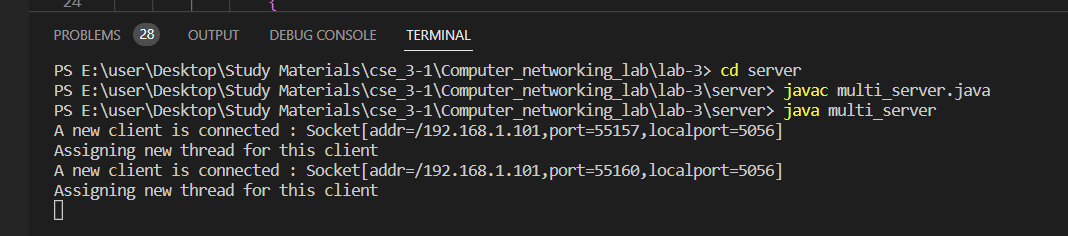
\includegraphics[width=\textwidth]{mserver.png}
\caption{Terminal output of server java file }
\end{figure}
\FloatBarrier


\textbf{Java implementation for Client}
Client-side programming is similar to general socket program with the following steps-
 \begin{itemize}
        
        \item Establish a Socket Connection

        \item Communication
\end{itemize}
Functioning steps of the entire program are : 
 \begin{itemize}
        \item When a client, say client1 sends a request to connect to server, the server assigns a new thread to handle this request. The newly assigned thread is given the access to streams for communicating with the client.
        \item After assigning the new thread, the server via its while loop, again comes into accepting state.
        \item When a second request comes while first is still in process, the server accepts this requests and again assigns a new thread for processing it. In this way, multiple requests can be handled even when some requests are in process.
\end{itemize}

\vspace{.5cm}
\textbf{Java code for client : }\\[12pt]
\begin{verbatim}
import java.io.*;
import java.net.*;
import java.util.Scanner;


public class multi_client
{
	public static void main(String[] args) throws IOException
	{
		try
		{
			Scanner scn = new Scanner(System.in);
			InetAddress ip = InetAddress.getByName("192.168.1.101");
			Socket s = new Socket(ip, 5056);
			DataInputStream dis = new DataInputStream(s.getInputStream());
			DataOutputStream dos = new DataOutputStream(s.getOutputStream());
			while (true)
			{
				System.out.println(dis.readUTF());
				String tosend = scn.nextLine();
				dos.writeUTF(tosend);
				if(tosend.equals("Exit"))
				{
					System.out.println("Closing this connection : " + s);
					s.close();
					System.out.println("Connection closed");
					break;
				}
				String received = dis.readUTF();
				System.out.println(received);
			}
			scn.close();
			dis.close();
			dos.close();
		}catch(Exception e){
			e.printStackTrace();
		}
	}
}
\end{verbatim}

 Output : 
  \begin{figure}[!h]
\centering
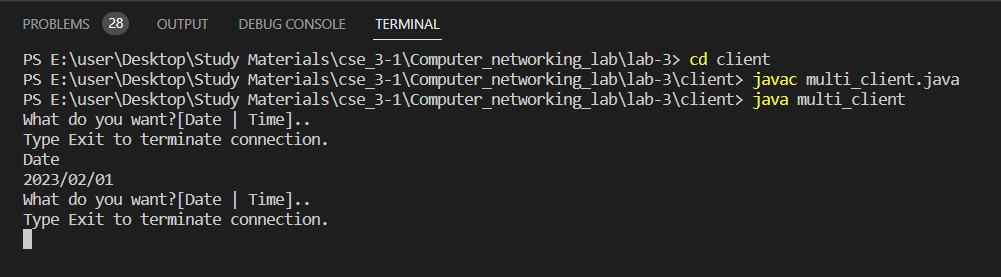
\includegraphics[width=\textwidth]{mclient.png}
\caption{Terminal output of client java file }
\end{figure}
\FloatBarrier



\subsubsection{Implementing file transferring via Socket Programming}

\vspace{.5cm}
\textbf{Java Implementation for server}\\[12pt]

\vspace{1cm}
\textbf{Java code for server : }\\[12pt]

\begin{verbatim}
import java.io.*;
import java.text.*;
import java.util.*;
import java.net.*;
public class file_socket_server
{
	

	private static DataInputStream dataInputStream;
	private static DataOutputStream dataOutputStream;

	

	public static void main(String[] args) throws IOException
	{
	
		ServerSocket ss = new ServerSocket(5010);
		
		while (true)
		{
			Socket s = null;
			
			try
			{
				s = ss.accept();
				
				System.out.println("A new client is connected : " + s);
				 dataInputStream= new DataInputStream(s.getInputStream());
				 dataOutputStream= new DataOutputStream(s.getOutputStream());
				
				System.out.println("Assigning new thread for this client");

				// create a new thread object
				Thread t = new ClientHandler(s, dataInputStream, dataOutputStream);
				t.start();
				
			}
			catch (Exception e){
                ss.close();
				s.close();
				e.printStackTrace();
			}
		}
	}
}

// ClientHandler class
class ClientHandler extends Thread
{
	
	static DataInputStream dis;
	static DataOutputStream dos;
	static Socket s;
	
	private static void receiveFile(String fileName)
		throws Exception
	{
		int bytes = 0;
		FileOutputStream fileOutputStream
			= new FileOutputStream(fileName);

		long size
			= dis.readLong(); // read file size
		byte[] buffer = new byte[4 * 1024];
		while (size > 0
			&& (bytes = dis.read(
					buffer, 0,
					(int)Math.min(buffer.length, size)))
					!= -1) {
			// Here we write the file using write method
			fileOutputStream.write(buffer, 0, bytes);
			size -= bytes; // read upto file size
		}
		fileOutputStream.close();
	}

	private static void sendFile(String path)
        throws Exception
    {
        int bytes = 0;
        File file = new File(path);
        FileInputStream fileInputStream
            = new FileInputStream(file);
        dos.writeLong(file.length());
        byte[] buffer = new byte[4 * 1024];
        while ((bytes = fileInputStream.read(buffer))
               != -1) {
          // Send the file to Server Socket 
          dos.write(buffer, 0, bytes);
            dos.flush();
        }
        fileInputStream.close();
    }

	// Constructor
	public ClientHandler(Socket s, DataInputStream dis, DataOutputStream dos)
	{
		this.s = s;
		this.dis = dis;
		this.dos = dos;
	}

	@Override
	public void run()
	{
		String received;
		while (true)
		{
			try {

				// Ask user what he wants
				dos.writeUTF("1. Type send to send the file\n2. Type receive to receive the file\n"+
							"Type Exit to terminate connection.");
				received = dis.readUTF();
				
				if(received.equals("Exit"))
				{
					System.out.println("Client " + this.s + " sends exit...");
					System.out.println("Closing this connection.");
					this.s.close();
					System.out.println("Connection closed");
					break;
				}
				else if(received.toLowerCase().equals("send"))
				{
					dos.writeUTF("Name of file: ");
					received=dis.readUTF();
					receiveFile(received);
					dos.writeUTF("File sent\n");
				}
				else if(received.toLowerCase().equals("receive"))
				{
					dos.writeUTF("Name of file: ");
					received=dis.readUTF();
					sendFile(received);
					dos.writeUTF("File received\n");
				}
				else
				{
					dos.writeUTF("Invalid Command");
				}

				
				
				
			} catch (Exception e) {
				e.printStackTrace();
			}
		}
		
		try
		{
			// closing resources
			this.dis.close();
			this.dos.close();
			
		}catch(IOException e){
			e.printStackTrace();
		}
	}
}
\end{verbatim}

 Output : 
\begin{figure}[!h]
\centering
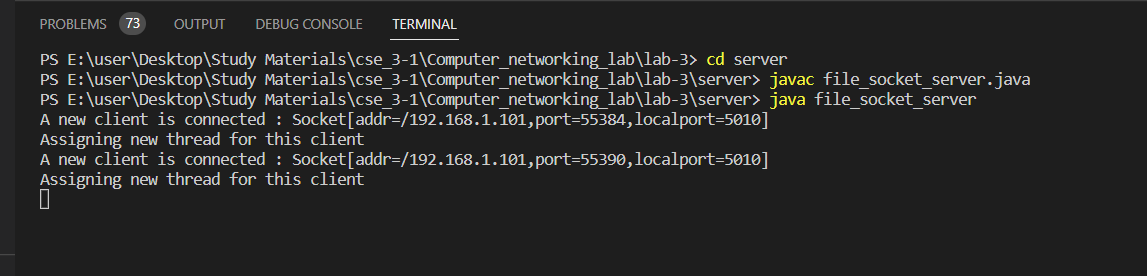
\includegraphics[width=\textwidth]{so_server.png}
\caption{Terminal output of server java file }
\end{figure}
\FloatBarrier

\textbf{Java Implementation for client}\\[12pt]

\vspace{1cm}
\textbf{Java code for client : }\\[12pt]
\begin{verbatim}
import java.io.*;
import java.net.Socket;
import java.util.Scanner;

public class file_socket_client {
	private static DataOutputStream dataOutputStream = null;
	private static DataInputStream dataInputStream = null;

	public static void main(String[] args)
	{
	
		try (Socket socket = new Socket("192.168.1.101", 5010)) {
			Scanner scn = new Scanner(System.in);
			
		dataInputStream = new DataInputStream(
				socket.getInputStream());
			dataOutputStream = new DataOutputStream(
				socket.getOutputStream());

		while (true)
			{
				System.out.println(dataInputStream.readUTF());
				String tosend = scn.nextLine();
				//System.out.println("W!");
				dataOutputStream.writeUTF(tosend);

				if(tosend.equals("Exit"))
				{
					System.out.println("Closing this connection : " + socket);
					socket.close();
					System.out.println("Connection closed");
					break;
				}

				System.out.println(dataInputStream.readUTF());

				if(tosend.toLowerCase().equals("send"))
				{
					tosend = scn.nextLine();
				    dataOutputStream.writeUTF(tosend);
					sendFile(tosend);
					
				}

				else if(tosend.toLowerCase().equals("receive"))
				{
					tosend = scn.nextLine();
					dataOutputStream.writeUTF(tosend);
					receiveFile(tosend);
				}

				String received = dataInputStream.readUTF();
				System.out.println(received);
			}
	

			dataInputStream.close();
			dataInputStream.close();
		}
		catch (Exception e) {
			e.printStackTrace();
		}
	}


	private static void sendFile(String path)
		throws Exception
	{
		int bytes = 0;
		// Open the File where he located in your pc
		File file = new File(path);
		FileInputStream fileInputStream
			= new FileInputStream(file);

		dataOutputStream.writeLong(file.length());
		// Here we break file into chunks
		byte[] buffer = new byte[4 * 1024];
		while ((bytes = fileInputStream.read(buffer))
			!= -1) {
		// Send the file to Server Socket
		dataOutputStream.write(buffer, 0, bytes);
			dataOutputStream.flush();
		}

		fileInputStream.close();
	}

	 private static void receiveFile(String fileName)
        throws Exception
    {
        int bytes = 0;
        FileOutputStream fileOutputStream
            = new FileOutputStream(fileName);
 
        long size
            = dataInputStream.readLong(); // read file size
        byte[] buffer = new byte[4 * 1024];
        while (size > 0
               && (bytes = dataInputStream.read(
                       buffer, 0,
                       (int)Math.min(buffer.length, size)))
                      != -1) {
            // Here we write the file using write method
            fileOutputStream.write(buffer, 0, bytes);
            size -= bytes; // read upto file size
        }
	    
        fileOutputStream.close();
    }
}
\end{verbatim}


 Output : 
\begin{figure}[!h]
\centering
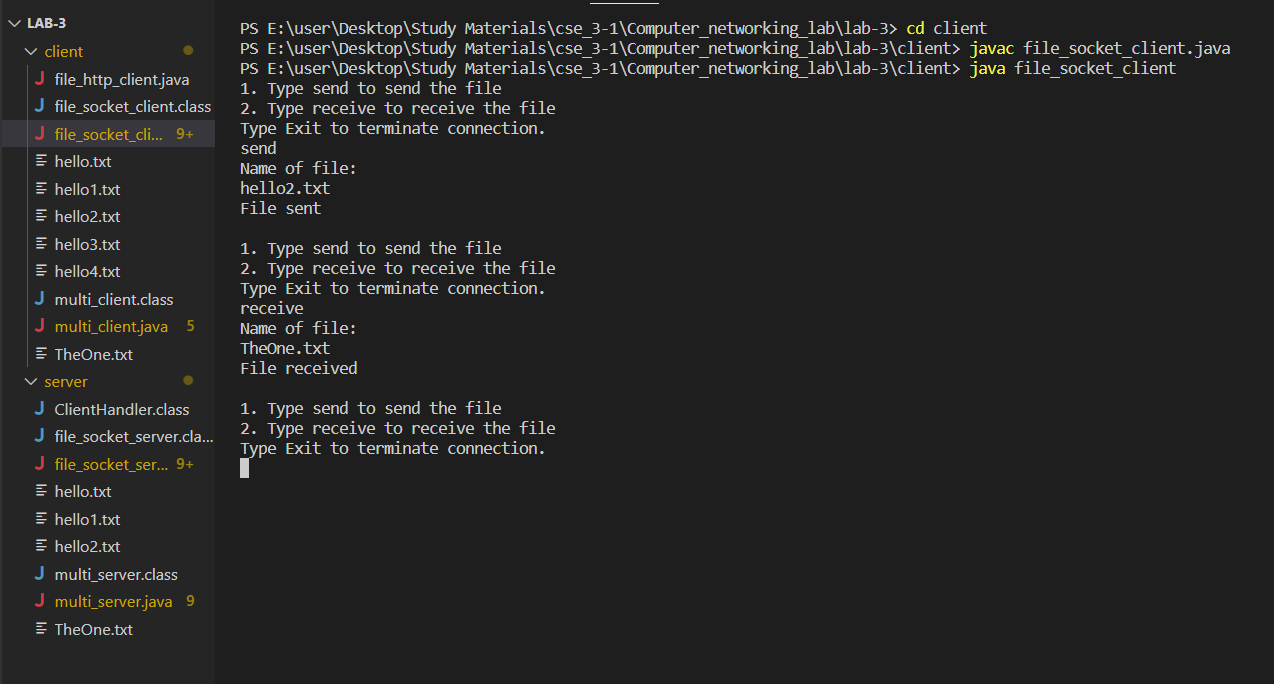
\includegraphics[width=\textwidth]{so_client.png}
\caption{Terminal output of client java file }
\end{figure}
\FloatBarrier

\subsection{File Transfer via HTTP}

An HTTP file transfer is the process of transferring a file between multiple nodes/devices using the HTTP protocol, or more generally, the Internet.

It is one of the most commonly used methods for sending, receiving or exchanging data and files over the Internet or a TCP/IP-based network.

\pagebreak
\textbf{Java Implementation for server side}\\[12pt]

\vspace{.5cm}

\textbf{Java code for server Controller file : }\\[12pt]
\begin{verbatim}
package com.example.server_http;
import org.springframework.http.HttpStatus;
import org.springframework.http.ResponseEntity;
import org.springframework.web.bind.annotation.*;
import org.springframework.web.multipart.MultipartFile;
import java.io.File;
import java.io.IOException;
import java.nio.file.Files;
import java.nio.file.Path;
import java.nio.file.Paths;
import java.nio.file.StandardCopyOption;
import java.util.Objects;

@RestController
public class Controller {
    private static final String FILE_UPLOAD_DIRECTORY = "./uploads/";

    @PostMapping("/post/")
    public ResponseEntity<String> saveFile(@RequestParam MultipartFile file){

        try{
            Path fileStorageLocation = Paths.get(FILE_UPLOAD_DIRECTORY).
            toAbsolutePath().normalize();
            Files.createDirectories(fileStorageLocation);
            Path targetLocation = fileStorageLocation.resolve
            (Objects.requireNonNull("uploaded"+System.currentTimeMillis()+file
            .getOriginalFilename()));
            Files.copy(file.getInputStream(), targetLocation, StandardCopyOption
            .REPLACE_EXISTING);
        }
        catch (IOException e){
            return ResponseEntity.status(HttpStatus.BAD_REQUEST)
            .body("File Save Failed");
        }
        return ResponseEntity.ok().body("File Saved Successfully");
    }

    @GetMapping("/get/{fileName}")
    public ResponseEntity<File> retrieveFile(@PathVariable String fileName){
        File file = new File(FILE_UPLOAD_DIRECTORY + fileName);
        return ResponseEntity.ok().body(file);
    }
}
\end{verbatim}
\vspace{.5cm}
\textbf{Java code for server Main file : }\\[12pt]
\begin{verbatim}

package com.example.server_http;

import org.springframework.boot.SpringApplication;
import org.springframework.boot.autoconfigure.SpringBootApplication;

@SpringBootApplication
public class ServerHttpApplication {

    public static void main(String[] args) {
        SpringApplication.run(ServerHttpApplication.class, args);
    }

}
\end{verbatim}

 Output : 
\begin{figure}[!h]
\centering
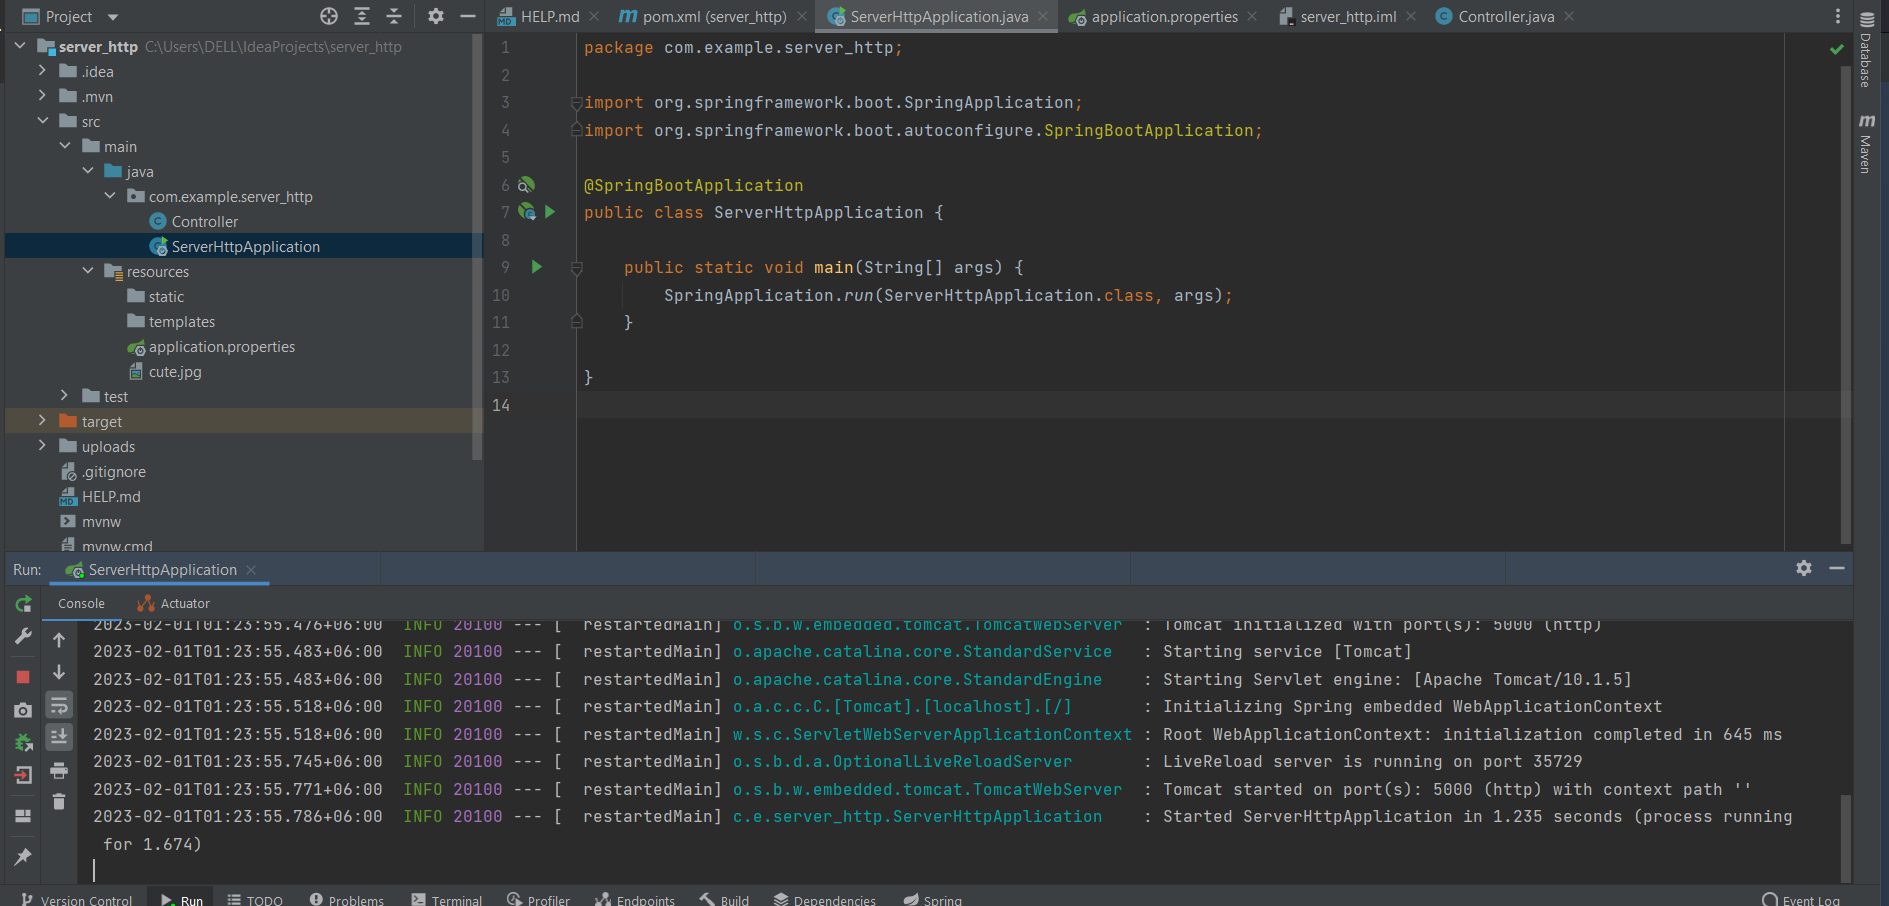
\includegraphics[width=\textwidth]{h_server.png}
\caption{Terminal output of server java file }
\end{figure}
\FloatBarrier

\pagebreak

\textbf{Java program for a Client : }\\[12pt]
\vspace{.5cm}
\textbf{Java code for a Client : }\\[12pt]
\begin{verbatim}
        import java.io.*;
        import java.net.HttpURLConnection;
        import java.net.URL;
        import java.nio.file.Files;
        import java.util.Scanner;

public class file_http_client{

    private static final String boundary =  "*****";
    private static final String space = "\r\n";
    private static final String gap = "--";
    private static Scanner scn;

    public static void main(String[] args) throws IOException {
        scn =new Scanner(System.in);
        while(true){
            System.out.println("Choose a Option\n1. POST (Uplaod file)\n2.
            GET (Download file)\n3. Exit");
            String userinp = scn.nextLine();
            switch (userinp){
                case "1":
                        filesendprompt();
                case "2":
                    filereceiveprompt();
                case "3":
                    System.out.println("You Successfully Exited");
                    return;
                default:
                    System.out.println("Wrong input. Try again please");
            }

        }
    }
    private static void filesendprompt() throws IOException {
        while (true)
        {
            System.out.println("Upload a file to the server \n1. hello1.txt\n2.
            hello2.txt\n3. hello3.txt\n4. hello4.txt\n5. Exit");
            String tosend = scn.nextLine();
            if(tosend.equals("1")){ filesend("hello1.txt");}
            else if(tosend.equals("2")){ filesend("hello2.txt");}
            else if(tosend.equals("3")){ filesend("hello3.txt");}
            else if(tosend.equals("4")){ filesend("hello4.txt");}
            else if(tosend.equals("5"))
            {
                return;
            }
            else{
                System.out.println("No such file found. Try again");
            }
        }

    }
    private static void filereceiveprompt() throws IOException {
        while (true)
        {
            System.out.println("Get file from server\n1. hello1.txt\n2. 
            hello2.txt\n3. hello3.txt\n4. hello4.txt\n5. Exit");
            String tosend = scn.nextLine();
            if(tosend.equals("1")){ fileget("hello1.txt");}
            else if(tosend.equals("2")){ fileget("hello2.txt");}
            else if(tosend.equals("3")){ fileget("hello3.txt");}
            else if(tosend.equals("4")){ fileget("hello4.txt");}
            else if(tosend.equals("5"))
            {
                return;
            }
            else{
                System.out.println("No such file found. Try again.");
            }
        }

    }
    private static void filesend(String filename) throws IOException {
        URL targetUrl = new URL("http://localhost:5000/post/");
        HttpURLConnection connection = (HttpURLConnection)
        targetUrl.openConnection();
        connection.setRequestMethod("POST");
        connection.setRequestProperty("Content-Type", "multipart/form-
        data;boundary=" + boundary); // Indicates file transmission
        connection.setDoOutput(true); // Indicates POST request
        DataOutputStream requestStream = new 
        DataOutputStream(connection.getOutputStream());
        String workingDirectory = System.getProperty("user.dir");
        String absoluteFilePath = "";
        absoluteFilePath = workingDirectory + File.separator + filename;
        File fileToSend = new File(absoluteFilePath);
        String fileName = fileToSend.getName();
        String fieldName = "file";
        requestStream.writeBytes(gap + boundary + space);
        requestStream.writeBytes("Content-Disposition: form-data; name=\"" +
                fieldName + "\";filename=\"" +
                fileName + "\"" + space);
        requestStream.writeBytes(space);

        byte[] fileBytes = Files.readAllBytes(fileToSend.toPath());
        requestStream.write(fileBytes);
        requestStream.writeBytes(space);
        requestStream.writeBytes(gap + boundary + gap + space);
        requestStream.flush();
        requestStream.close();

        int responseCode = connection.getResponseCode();
        System.out.println("POST Response Code: " + responseCode);

        if (responseCode == HttpURLConnection.HTTP_OK) { //success
            BufferedReader responseReader = new BufferedReader(new 
            InputStreamReader(connection.getInputStream()));
            String inputLine;
            StringBuilder response = new StringBuilder();

            while ((inputLine = responseReader.readLine()) != null) {
                response.append(inputLine);
            }
            responseReader.close();
            System.out.println(response+ "\nFile Saved to uploads folder!");
        }
        else {
            System.out.println("POST request did not succeed.");
        }
    }
    private static void fileget(String filename) throws IOException {
        String url = "http://localhost:5000/get/"+filename;
        URL obj = new URL(url);
        HttpURLConnection conn = (HttpURLConnection) obj.openConnection();
        conn.setRequestMethod("GET");
        int responseCode = conn.getResponseCode();
        System.out.println("GET Response Code: " + responseCode);
        if (responseCode == HttpURLConnection.HTTP_OK) {
            String fileName = extractFileName(conn, url);
            InputStream inputStream = conn.getInputStream();
            String workingDirectory = System.getProperty("user.dir");
            String saveFilePath = workingDirectory + File.separator + 
            "received"+System.currentTimeMillis()+fileName;
            FileOutputStream outputStream = new FileOutputStream(saveFilePath);
            int bytesRead;
            byte[] buffer = new byte[400096];
            while ((bytesRead = inputStream.read(buffer)) != -1) {
                outputStream.write(buffer, 0, bytesRead);
            }
            outputStream.close();
            inputStream.close();
            System.out.println("File downloaded from server");
        } else {
            System.out.println("GET request did not worked");
        }
    }

    private static String extractFileName(HttpURLConnection conn, String url) {
        String fileName = "";
        String disposition = conn.getHeaderField("Content-Disposition");
        if (disposition != null) {
            int index = disposition.indexOf("filename=");
            if (index > 0) {
                fileName = disposition.substring(index + 10,
                        disposition.length() - 1);
            }
        } else {
            fileName = url.substring(url.lastIndexOf("/") + 1);
        }
        return fileName;
    }

}
\end{verbatim}




 Output For POST: 
\begin{figure}[!h]
\centering
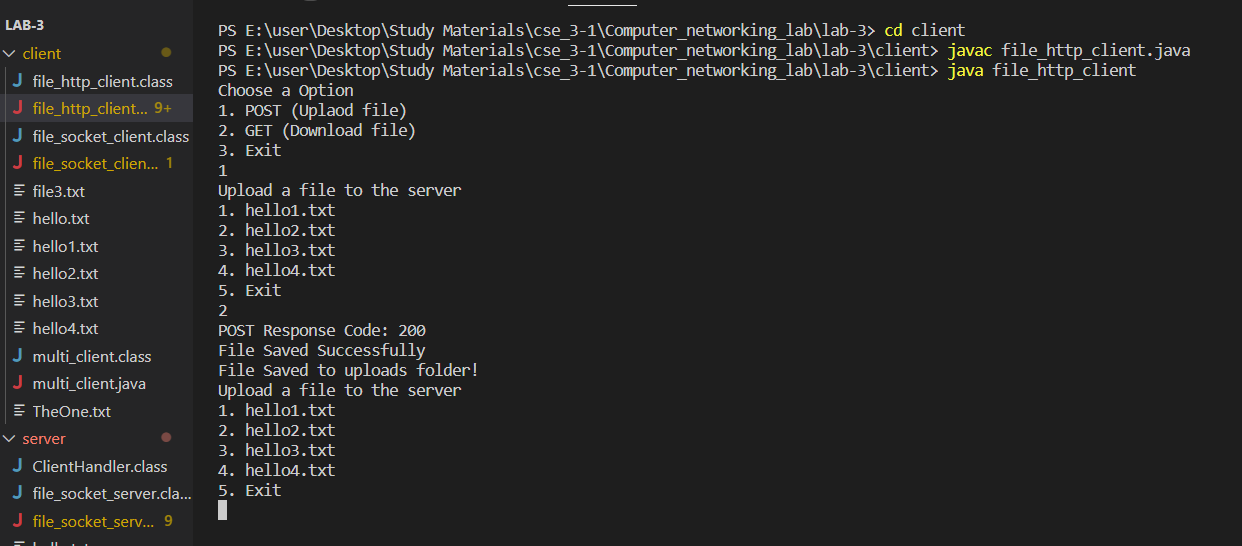
\includegraphics[width=\textwidth]{post_client.png}
\caption{Terminal output of client java file for post }
\end{figure}
\FloatBarrier

 Output For GET : 
\begin{figure}[!h]
\centering
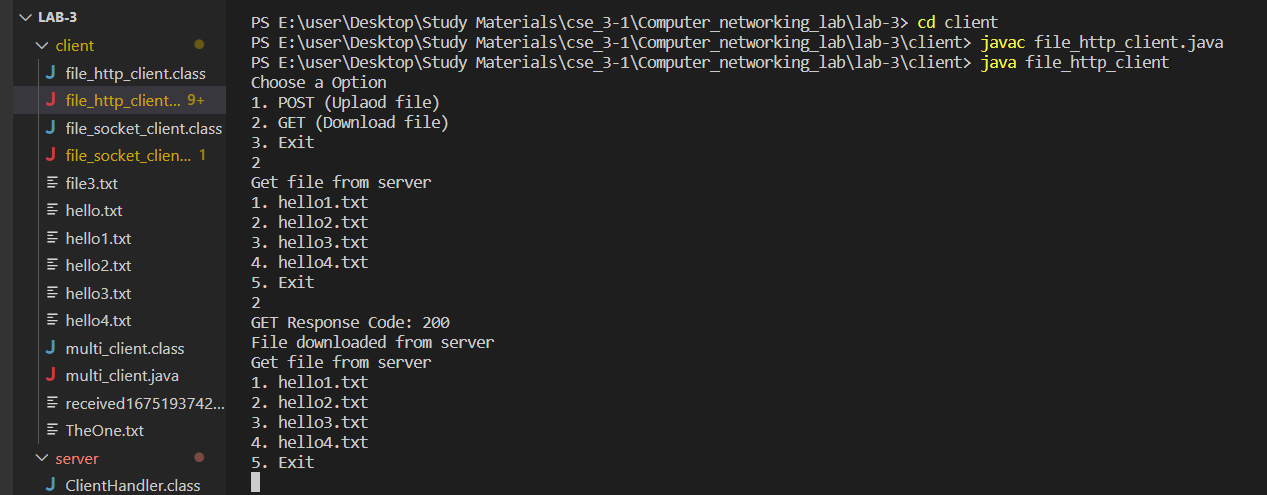
\includegraphics[width=\textwidth]{get_client.png}
\caption{Terminal output of client java file for get }
\end{figure}
\FloatBarrier




\section{Experience}
\begin{enumerate}
   \item Here we have learned about file transferring via TCP socket programming.
    \item We have come to know about how with the help of HTTP we can also transfer files.
\end{enumerate}
\begin{thebibliography}{1}
\bibitem{chat}  Chat with multiple clients :\url{https://www.geeksforgeeks.org/introducing-threads-socket-programming-java}
\bibitem{socket} File Transfer via socket: \url{https://www.geeksforgeeks.org/transfer-the-file-client-socket-to-server-socket-in-java/}
\bibitem{getpost} Sending GET/POST requests : \url{https://www.digitalocean.com/community/tutorials/java-httpurlconnection-example-java-http-request-get-post}
\end{thebibliography}
\end{document}
